\documentclass[10pt]{article}
\usepackage[pdftex]{graphicx}
\usepackage{multicol}
\usepackage{float}
\usepackage{caption}
\hyphenation{op-tical net-works semi-conduc-tor auto-nomous magneto-meter}
\setlength{\topmargin}{0in}
\setlength{\headheight}{0in}
\setlength{\headsep}{0in}
\setlength{\textheight}{10in}
\setlength{\textwidth}{6.5in}
\setlength{\oddsidemargin}{0in}
\setlength{\evensidemargin}{0in}
\setlength{\parindent}{0.25in}
\pagestyle{empty}
\begin{document}
\title{2010 AUVSI UAS Competition: Fact Sheet}
\author{Rutgers Autonomous Aircraft Team
\\President: Anthony Garrison
\\Aero Design Team Leader: Greg Quinn
\\Electronics Design Team Leader: Pat Hickey}
\begin{center}
{\huge \bfseries 2010 AUVSI UAS Competition: Fact Sheet } \\[0.5cm]
{\large \bfseries Rutgers University Autonomous Aircraft Team } \\[0.5cm]
{President: Anthony Garrison \\ Aircraft Design Team Leader: Greg Quinn
\\Electronics Design Team Leader: Pat Hickey
\\Correspondence: pchickey@eden.rutgers.edu}\\
\end{center}

\begin{figure}[b]
  \centering
    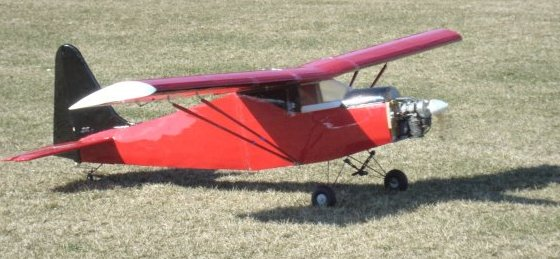
\includegraphics[width=0.4\textwidth]{../images/daedalus.jpg}
  \captionsetup{width=.70\textwidth}
  \caption{The Daedalus. Maiden flight on 18 March 2010 available at http://bit.ly/RUdaedalus}
\end{figure}
\begin{multicols}{2}
\section{Airframes}
We have two similar airframes for crash redundancy. The flight electronics and payload are modular. We use the same payload and radio equipment in each airframe.
\subsection{Daedalus}
\emph{Maiden Flight 18 March 2010}
\\Model: 10ft Custom Built Cessna
\\Wingspan: 10ft
\\Length: 6ft
\\Gross Weight: 27lb
\\Engine: 45cc two-stroke gasoline
\\Fuel: Gasoline with two stroke oil
\\Fuel Capacity: 24oz
\\Propeller: 22in (56cm) diameter
\\Battery: 7.2v 2.4Ah Lithium Polymer
\subsection{12ft Telemaster}
\emph{Under Construction}
\\Model: Aero Craft Ltd. 12ft Telemaster
\\Wingspan: 12ft
\\Length: 7ft 6in
\\Gross Weight: 27lb
\\Engine: Fuji-Imvac BT-43EI 43cc
\\Fuel: Gasoline with two stroke oil
\\Fuel Capacity: 24oz
\\Propeller: 22in (56cm) diameter
\\Battery: 7.2v 2.4Ah Lithium Polymer

\section{Autonomous Control}
Autopilot: Paparazzi Autopilot for Linux
\\Hardware: Beagleboard Single Board Computer
\\Battery: 11.1v 1.5Ah Lithium Polymer
\subsection{Sensors}
GPS: uBlox LEA-5H based 
\\IMU: Custom three-axis Accellerometer, Magnetometer, and Rate Gyro

\section{Payload}
Camera: Sony MHS-PM5
\\Resolution: 5MP
\\Pan-Tilt unit: 120 degree tilt, 720 degree pan

\section{Radio Systems}
\subsection{R/C Saftey Radio Link}
Futaba 2.4GHz FAAST 6 channel radio system
\\Frequency Band: 2.4GHz
\subsection{Autopilot Long Range Telemetry}
Maxstream XBee Pro Series 2.5
\\Frequency Band: 2.4GHz
\subsection{Autopilot Wifi Telemetry}
802.11n 5GHz Router and USB Adapter
\\Frequency Band: 5GHz
\subsection{Video Downlink}
RangeVideo TX-900 500mW Video Transmitter
\\Frequency Band: 900MHz
\\Power: 500mW
\\License: FCC Amateur Radio Technician

\end{multicols}

\end{document}


